%
% @author   Shmish  "shmish90@gmail.com"
% @legal    MIT     "(c) Christopher Schmitt"
%


\documentclass{article}


%
% Document Imports
%

\usepackage{fancyhdr}
\usepackage{extramarks}
\usepackage{amsmath}
\usepackage{amssymb}
\usepackage{amsthm}
\usepackage{amsfonts}
\usepackage{color}
\usepackage{tikz}
\usepackage{listings}



%
% Document Configuration
%

\newcommand{\hwAuthor}{Christopher K. Schmitt}
\newcommand{\hwSubject}{CS 483}
\newcommand{\hwSection}{Section 01}
\newcommand{\hwSemester}{Fall 2020}
\newcommand{\hwAssignment}{Assignment 2}

\usetikzlibrary{arrows,automata}


%
% Document Environments
%

\setlength{\headheight}{65pt}
\pagestyle{fancy}
\lhead{\hwAuthor}
\rhead{
  \hwSubject \\
  \hwSection \\
  \hwSemester \\
  \hwAssignment
}

\newenvironment{problem}[1]{
  \nobreak\section*{Problem #1}
}{}


%
% Document Start
%

\begin{document}
  \begin{problem}{1}
    \textbf{DFA1:}
    \begin{center}
      \begin{tikzpicture}[>=stealth',shorten >=1pt,auto,node distance=2cm]
        \node[state, initial] (q0) {$q_0$};
        \node[state] (q1) [below of = q0] {$q_1$};
        \node[state] (q2) [right of = q0] {$q_2$};
        \node[state, accepting] (q3) [right of = q2] {$q_3$};

        \path[->] (q0) edge node {$0$} (q1);
        \path[->] (q1) edge[loop right] node {$0, 1$} (q1);
        \path[->] (q0) edge node {$1$} (q2);
        \path[->] (q2) edge[bend left] node {$0$} (q3);
        \path[->] (q2) edge[loop above] node {$1$} (q2);
        \path[->] (q3) edge[bend left] node {$1$} (q2);
        \path[->] (q3) edge[loop above] node {$0$} (q3);
      \end{tikzpicture}
    \end{center}

    \begin{center}
      \includegraphics[scale=0.5]{images/DFA1_ACCEPTED.jpg}
      \includegraphics[scale=0.5]{images/DFA1_REJECTED.jpg}
    \end{center}

    \pagebreak
    \noindent
    \textbf{DFA2:}
    \begin{center}
      \begin{tikzpicture}[>=stealth',shorten >=1pt,auto,node distance=2cm]
        \node[state, initial] (q0) {$q_0$};
        \node[state] (q1) [right of = q0] {$q_1$};
        \node[state] (q2) [right of = q1] {$q_2$};
        \node[state, accepting] (q3) [right of = q2] {$q_3$};

        \path[->] (q0) edge node {$1$} (q1);
        \path[->] (q1) edge node {$1$} (q2);
        \path[->] (q2) edge node {$1$} (q3);

        \path[->] (q0) edge[loop above] node {$0$} (q0);
        \path[->] (q1) edge[loop above] node {$0$} (q1);
        \path[->] (q2) edge[loop above] node {$0$} (q2);
        \path[->] (q3) edge[loop above] node {$0, 1$} (q3);
      \end{tikzpicture}
    \end{center}

    \begin{center}
      \includegraphics[scale = 1]{images/DFA2_ACCEPTED.jpg}
      \includegraphics[scale = 1]{images/DFA2_REJECTED.jpg}
    \end{center}

    \pagebreak
    \noindent
    \textbf{NFA1:}
    \begin{center}
      \begin{tikzpicture}[>=stealth',shorten >=1pt,auto,node distance=2cm]
        \node[state, initial] (q0) {$q_0$};
        \node[state] (q1) [right of = q0] {$q_1$};
        \node[state, accepting] (q2) [right of = q1] {$q_2$};

        \path[->] (q0) edge node {$1$} (q1);
        \path[->] (q1) edge node {$0$} (q2);
        \path[->] (q1) edge[loop above] node {$0, 1$} (q1);
      \end{tikzpicture}
    \end{center}

    \begin{center}
      \includegraphics[scale = 1]{images/NFA1_ACCEPTED.jpg}
      \includegraphics[scale = 1]{images/NFA1_REJECTED.jpg}
    \end{center}

    \pagebreak
    \noindent
    \textbf{NFA2:}
    \begin{center}
      \begin{tikzpicture}[>=stealth',shorten >=1pt,auto,node distance=2cm]
        \node[state, initial] (q0) {$q_0$};
        
        \node[state] (q1) [below right of = q0] {$q_1$};
        \node[state] (q2) [right of = q1] {$q_2$};
        \node[state] (q3) [right of = q2] {$q_3$};
        \node[state, accepting] (q4) [right of = q3] {$q_4$};

        \node[state] (q5) [above right of = q0] {$q_5$};
        \node[state] (q6) [above of = q5] {$q_6$};
        \node[state] (q7) [right of = q5] {$q_7$};
        \node[state, accepting] (q8) [right of = q7] {$q_8$}; 

        \path[->] (q0) edge node {$\epsilon$} (q1);
        \path[->] (q1) edge node {$1$} (q2);
        \path[->] (q2) edge node {$1$} (q3);
        \path[->] (q3) edge node {$1$} (q4);

        \path[->] (q1) edge[loop below] node {$0$} (q1);
        \path[->] (q2) edge[loop below] node {$0$} (q2);
        \path[->] (q3) edge[loop below] node {$0$} (q3);
        \path[->] (q4) edge[loop below] node {$0, 1$} (q4);

        \path[->] (q0) edge node {$\epsilon$} (q5);
        \path[->] (q5) edge node {$0$} (q6);
        \path[->] (q6) edge[loop left] node {$0, 1$} (q6);
        \path[->] (q5) edge node {$1$} (q7);
        \path[->] (q7) edge[loop above] node {$1$} (q7);
        \path[->] (q7) edge[bend left] node {$0$} (q8);
        \path[->] (q8) edge[bend left] node {$1$} (q7);
        \path[->] (q8) edge[loop above] node {$0$} (q8);
      \end{tikzpicture}
    \end{center}
  \end{problem}

  \begin{problem}{2}
    \lstinputlisting[language=Java, basicstyle=\footnotesize]{Main.java}
    \includegraphics{images/Regex.jpg}
  \end{problem}

  \begin{problem}{3}
    \begin{center}
      \begin{tikzpicture}[>=stealth',shorten >=1pt,auto,node distance=2cm]
        \node[state, initial] (q0) {$q_0$};
        \node[state] (q1) [right of = q0] {$q_1$};
        \node[state, accepting] (q2) [right of = q1] {$q_2$};
        \node[state] (q3) [right of = q2] {$q_3$};

        \path[->] (q0) edge node {$1$} (q1);
        \path[->] (q1) edge node {$0$} (q2);
        \path[->] (q2) edge[loop below] node {$0$} (q2);
        \path[->] (q2) edge[bend left] node {$1$} (q3);
        \path[->] (q3) edge[bend left] node {$0$} (q2);
        \path[->] (q3) edge[loop right] node {$1$} (q3);
        \path[->] (q1) edge[bend left] node {$1$} (q3);
      \end{tikzpicture}
    \end{center}

    \begin{center}
      \includegraphics[scale = 1]{images/Regex_ACCEPTED.jpg}
      \includegraphics[scale = 1]{images/Regex_REJECTED.jpg}
    \end{center}
  \end{problem}
\end{document}